\documentclass[11pt]{article}
\usepackage[english]{babel}
\usepackage[utf8]{inputenc}
\usepackage{amsmath,amsthm,amssymb,graphicx,pdfpages,lipsum,hyperref}
\usepackage[none]{hyphenat}
\setlength\parindent{0pt}
\usepackage[top=0.9in, left=0.9in, bottom=0.9in, right=0.9in]{geometry}
%%%%%%%%%%%%%%%%%%%%%%%%%%%%%%%%%%%%%%%%%%%%%%%%%%%%%%%%%%%%%%%%%%%
% add other packages here if required
\usepackage[export]{adjustbox}
\usepackage{subcaption}
\usepackage{wrapfig}

\title{Chiller parts expected fault date prediction and visualization}
\author{Yuxin Ma\\
        Bangguo Wei\\
        }
\date{\today}

\begin{document}

\maketitle

\tableofcontents

\newpage

\section{Business background}

The company finds it’s costly to arrange a worker to repair a chiller without knowing which parts are failed inside. The worker will have an issue identifying what parts to bring when scheduling their repair job and is time-consuming to fetch the broken parts twice. Only (53) percent of all repairs that required component parts were wrapped up with a single visit, and It costs about (\$6.49) to return every single unnecessary part to a warehouse. The algorithms in this project are aimed to identify what parts failed during a period and to offer reliable guidance to repair workers. The project is set up to mitigate the inefficiency issue just raised above, thus improving the workers' productivity and improving the company's profit in the long run.

\section{Machine Learning model}

\subsection{Framework}

\subsubsection{Data}
The original data set is confidential and is provided by the business team. The records contain 2 sample chillers, one chiller includes 43 parts, and the other includes 34 parts. For each part, we could obtain part description, identical part code, quantity, expected functioning hours and expected life cycle in years.

\subsubsection{Preprocess}
Before fitting into the models, we first expanded the parts that have more than one quantity. Then for more direct visualizations, a randomized start functioning date is simulated.

\subsubsection{Plan}
Predicted parts' life cycles are added up to each part's start functioning date. 

\subsection{Models}
We use the lifelines library in the Python library to analyze the product life distribution and predict the likelihood of an incoming replacement. So it's helpful for the company to prepare enough inventory and maintenance teams in advance.

\subsubsection{Training data labels}
For this supervised training, we need labels for training data. We set parts' life to label the original features data. We will give higher life scores when the outcome of the prediction is better.  

\subsubsection{Kaplan-Meier survival analysis}

Kaplan-Meier curve is a non-parametric statistic used to estimate the survival function from lifetime data, and we use the Kaplan-Meier curve to display how survival rates of the parts have changed in the figure 1 below. The horizontal axis in the figure 1 represents time, the vertical axis on the left represents survival probability, and the vertical axis on the right represents cumulative density. The figure shows that the median survival time of parts is 1269 days and the median survival confidence interval is between 865 and 1486 days.

\begin{figure}[h]
\begin{subfigure}{0.5\textwidth}
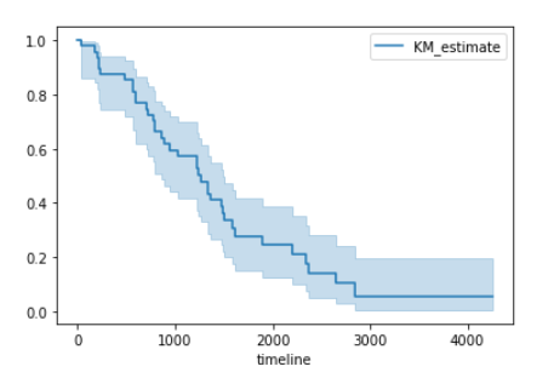
\includegraphics[width=0.9\linewidth, height=6cm]{KMF1.png} 
\caption{Survival Function}
\label{fig:subim1}
\end{subfigure}
\begin{subfigure}{0.5\textwidth}
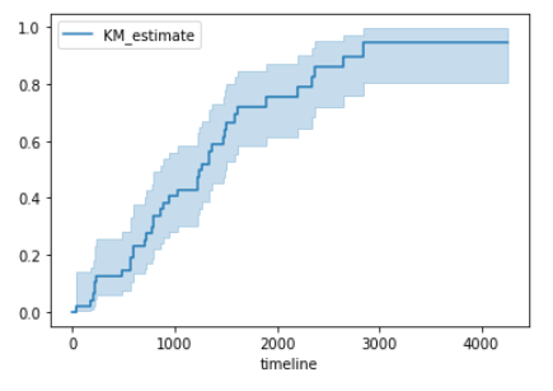
\includegraphics[width=0.9\linewidth, height=6cm]{KMF2.png}
\caption{Cumulative Density}
\label{fig:subim2}
\end{subfigure}
\caption{Kaplan-Meier curve for Parts life}
\label{fig:image2}
\end{figure}

\subsubsection{Wei-bull distribution}
In probability theory and statistics, the Weibull distribution is a continuous probability distribution that can fit an extensive range of distribution shapes. So we also use the Weibull distribution to fit the survival time probability of the part in Figure 2 below. The horizontal axis in figure 2 represents time, the vertical axis represents survival probability. The result in figure 2 shows the median survival time of parts is 1216 days and the Weibull mean survival time is  1486 days. The result is very similar to the Kaplan-Meier survival analysis.

\begin{figure}[h]
\centering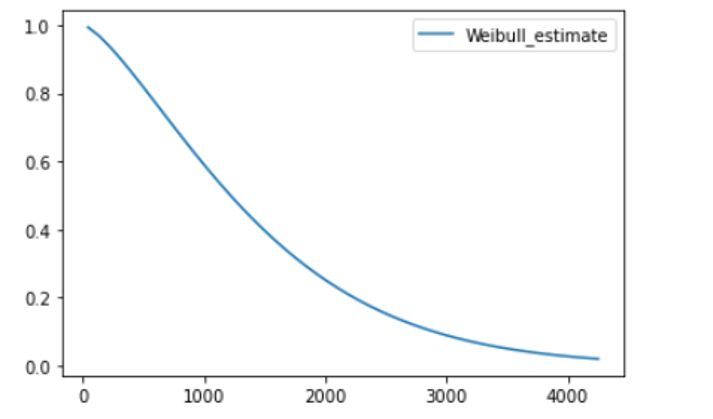
\includegraphics[width=0.8\linewidth, height=7cm]{Weibull.png} 
\caption{Weibull distribution estimate}
\end{figure}

\subsubsection{Model extraction}
When predicting part life, the output of the Weibull model is that each part increases with time, and the probability of part survival changes, so by setting a probability threshold, we can predict whether a part is normal or at risk of damage. On the other hand, we can adjust the probability threshold to control the range of parts that are detected as risky.
To evaluate our model, we use the AIC (Akaike information criterion) in the Lifelines library to judge the performance of the model, and perform statistical analysis (as shown in the figure below).

\begin{figure}[h]
\centering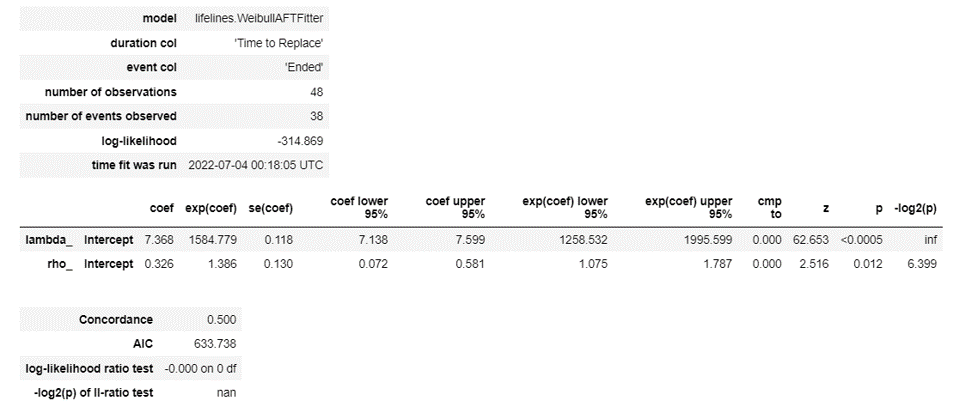
\includegraphics[width=0.8\linewidth, height=7cm]{Extraction_model.png} 
\caption{Weibull model fitting results}
\end{figure}

\subsection{Visualisation with Dash}
\subsubsection{Introducing Dash}
We visualized the expected fault time for each part using the Dash package in python. The interactive dashboard by Dash package allows users to check their targeted information by simply hovering the mouse and filtering.
\subsubsection{Functions}
The expected parts’ life cycles are obtained from the Wei-bull distribution described above. After adding on the start functioning date of each part, we could visualize the predicted fault date as in Figure 4 below. The x-axis shows when a part is about to fail while the y-axis indicates the identical part code. We could click on the dots in the graph to see each part's details, including part code, which chiller it belongs to, expected fail date, and description.
\\
The table below the plot contains detailed information associated with each part. It clarifies the details, and thus offers a more precise and translucent display to the users by scrolling down the cursor. 
\\
%\newpage
\begin{figure}[h]
\centering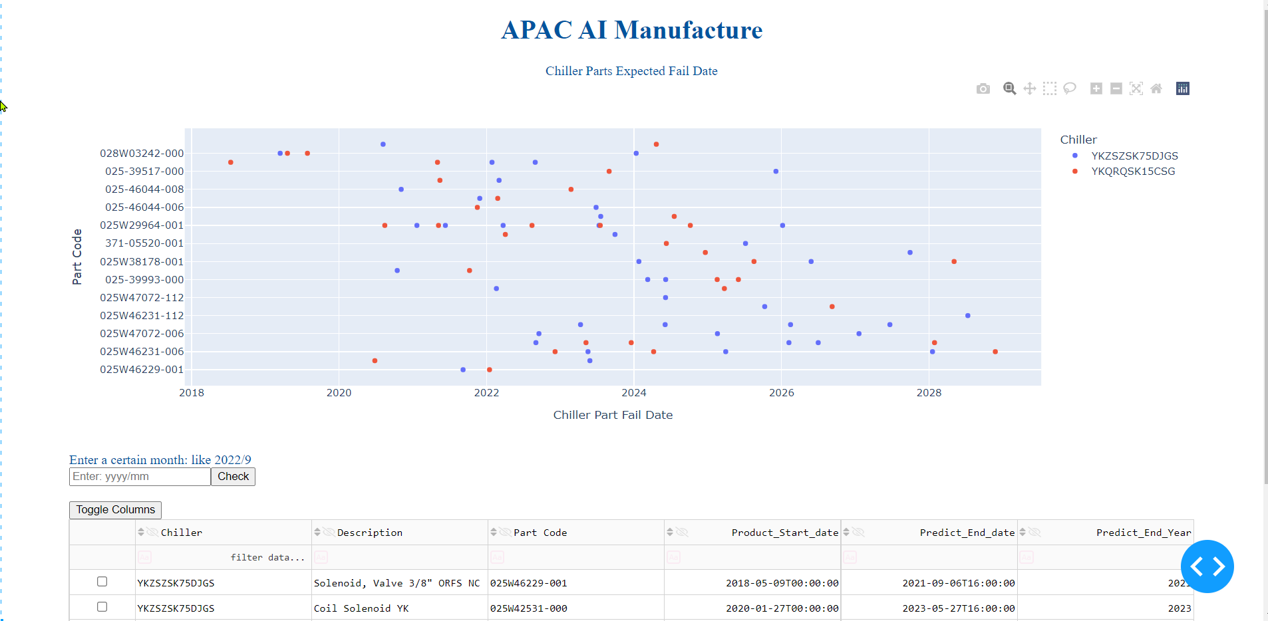
\includegraphics[width=0.8\linewidth, height=7cm]{Chillerparts_dateoverview.png} 
\caption{Chiller parts fault date overview}
\end{figure}
\\
The text box below the plot allows users to input a certain month with the format 'YYYY/MM'. Click on the 'Check' button, it can return which parts are expected to fail at the indicated point of time. The following figures show two possible scenarios when users input months correctly.
\\
\begin{figure}[h]
\begin{subfigure}{0.5\textwidth}
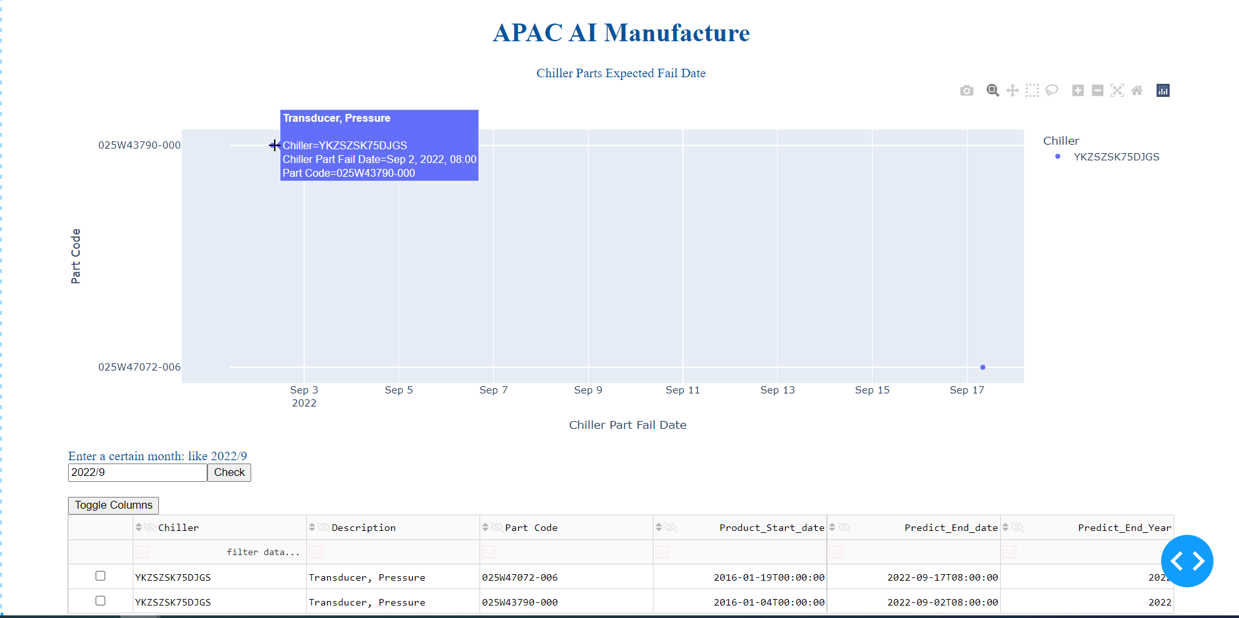
\includegraphics[width=0.9\linewidth, height=6cm]{partsfound.png} 
\caption{Parts about to fail}
\label{fig:subim1}
\end{subfigure}
\begin{subfigure}{0.5\textwidth}
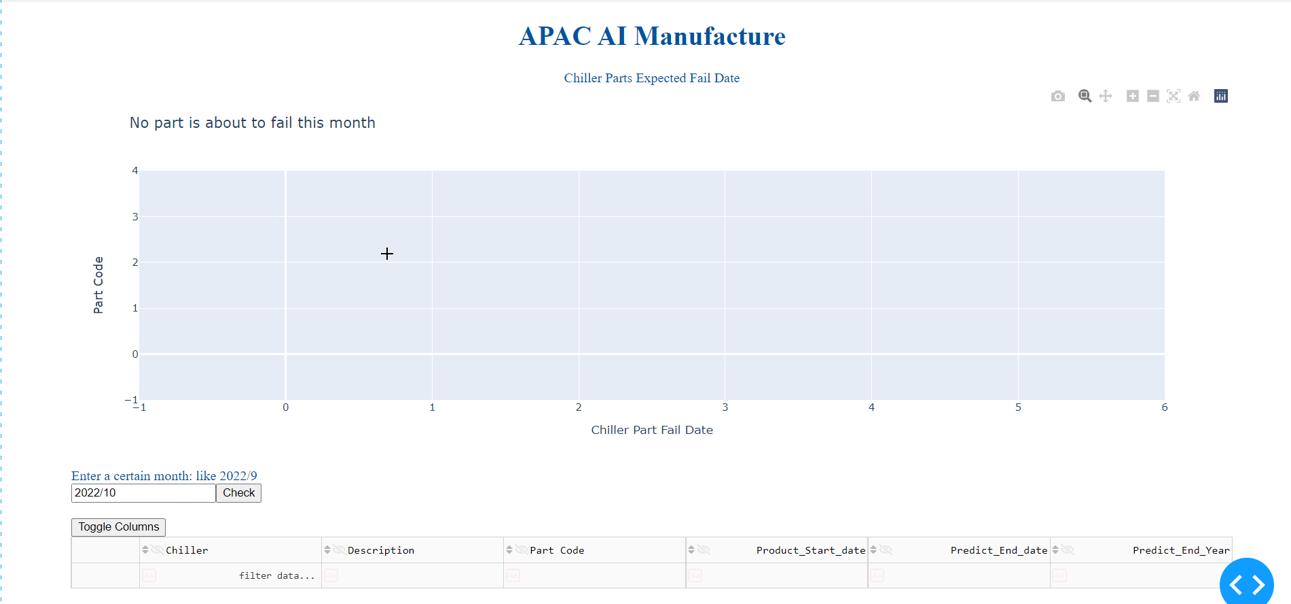
\includegraphics[width=0.9\linewidth, height=6cm]{nopartfound.png}
\caption{No part is about to fail}
\label{fig:subim2}
\end{subfigure}
\caption{Two possible scenarios with user input}
\label{fig:image2}
\end{figure}

\section{Business impact}
The business impact of the model is estimated as follows.
\\
 \textbf{Savings}: When a part reaches a critical life, we can try to monitor it through the dynamic interactive web page, check the life of the part in time, and provide effective suggestions for the exchange of parts (Note: the results are adopted by the commercial sector).

\end{document}